
\documentclass{article}
%encoding
%--------------------------------------
\usepackage[utf8]{inputenc}
\usepackage[T1]{fontenc}
%--------------------------------------
 
%German-specific commands
%--------------------------------------
\usepackage[ngerman]{babel}
\usepackage{csquotes}
%--------------------------------------

%Pictures
%--------------------------------------
\usepackage{graphicx}
\graphicspath{ {./Pictures/} }
\usepackage{tikz}
\usepackage{subcaption}
\usepackage{float}
\usepackage{wrapfig}
%--------------------------------------

%math
%--------------------------------------
\usepackage{amsmath}
\usepackage{amssymb}
\usepackage{amsfonts}
%--------------------------------------

%Frames
%--------------------------------------
\usepackage{framed}

%Colors
%--------------------------------------
\usepackage{xcolor}
\definecolor{blue-violet}{rgb}{0.54, 0.17, 0.89}
\definecolor{codegreen}{rgb}{0,0.6,0}
\definecolor{codegray}{rgb}{0.5,0.5,0.5}
\definecolor{codepurple}{rgb}{0.58,0,0.82}
\definecolor{backcolour}{rgb}{0.95,0.95,0.92}

%--------------------------------------
\usepackage{multicol}
\usepackage[shortlabels]{enumitem}

%Xsim
%--------------------------------------
\usepackage{xsim}
\DeclareExerciseType{example}{
exercise-env      = example,
solution-env      = examplesolution,
exercise-name     = \XSIMtranslate{example},
exercises-name    = \XSIMtranslate{examples},
solution-name     = \XSIMtranslate{solution},
solutions-name    = \XSIMtranslate{solutions},
exercise-template = default,
solution-template = default,
exercise-heading  = \subsection*,
solution-heading  = \subsection*
}
\DeclareExerciseTranslations{example}{
Fallback = example ,
English  = example ,
French   = example ,
German   = Beispiel
}
\DeclareExerciseType{question}{
exercise-env      = question,
solution-env      = questionsolution,
exercise-name     = \XSIMtranslate{question},
exercises-name    = \XSIMtranslate{questions},
solution-name     = \XSIMtranslate{solution},
solutions-name    = \XSIMtranslate{solutions},
exercise-template = default,
solution-template = default,
exercise-heading  = \subsection*,
solution-heading  = \subsection*
}
\DeclareExerciseTranslations{question}{
Fallback = question ,
English  = question ,
German   = Aufgabe
}


%Aufgaben
%--------------------------------------
% \usepackage{amsthm}
%\newtheorem{aufgabe}{Aufgabe}[section]
%\newtheorem{definition}{Definition}[section]
% \newtheorem{beispiel}{Beispiel}[section]
%--------------------------------------

%Listings
%--------------------------------------
\usepackage{ulem}
\usepackage{listings}
 
\lstdefinestyle{mystyle}{
    backgroundcolor=\color{backcolour},   
    commentstyle=\color{codegreen},
    keywordstyle=\color{magenta},
    numberstyle=\tiny\color{codegray},
    stringstyle=\color{codepurple},
    basicstyle=\ttfamily\footnotesize,
    breakatwhitespace=false,         
    breaklines=true,                 
    captionpos=b,                    
    keepspaces=true,                 
    numbers=left,                    
    numbersep=5pt,                  
    showspaces=false,                
    showstringspaces=false,
    showtabs=false,                  
    tabsize=2,
}
 
\lstset{style=mystyle,moredelim=[is][\sout]{|}{|}}
%--------------------------------------



\title{Einführung in die Automatentheorie}
\author{Alexandra Maximova}
\date{Oktober 2020}

\begin{document}

\maketitle

\begin{figure}[H]
\centering
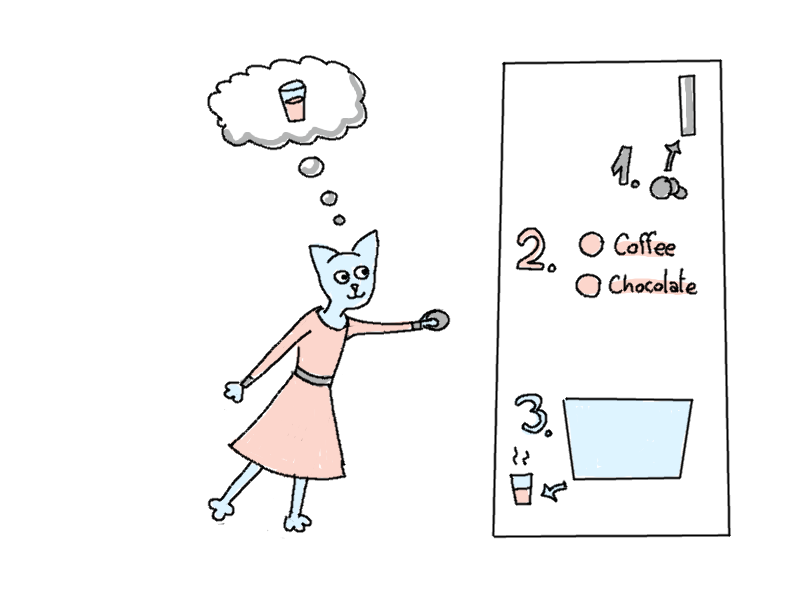
\includegraphics[width=\linewidth]{Pictures/image.png} 
\end{figure}


\section{Einführung}
Im Alltag interagieren wir mit vielen Maschinen, die sehr einfache Programme ausführen. Zum Beispiel, wie viele von euch haben heute den Lift genommen? Oder mussten an einer Ampel anstehen? Oder haben ein Getränk aus dem Automaten vor der Mensa genommen? Wie werden diese Gegenstände gesteuert?

Diese einfache Programme, die keine Variablen und keine Datenablage benötigen, nennt man \emph{endliche Automaten}. Heute werden wir Beispiele von endlichen Automaten kennenlernen und diesen Begriff genau mathematisch definieren. Auf dieser Basis werden wir dann in den nächsten Wochen aufbauen und beweisen, welche Probleme lassen sich mit solchen Programmen lösen und welche nicht.
\begin{example}
Das Beispiel mit der Ampel -- ausschreiben und zeichnen
\begin{figure}[H]
\centering
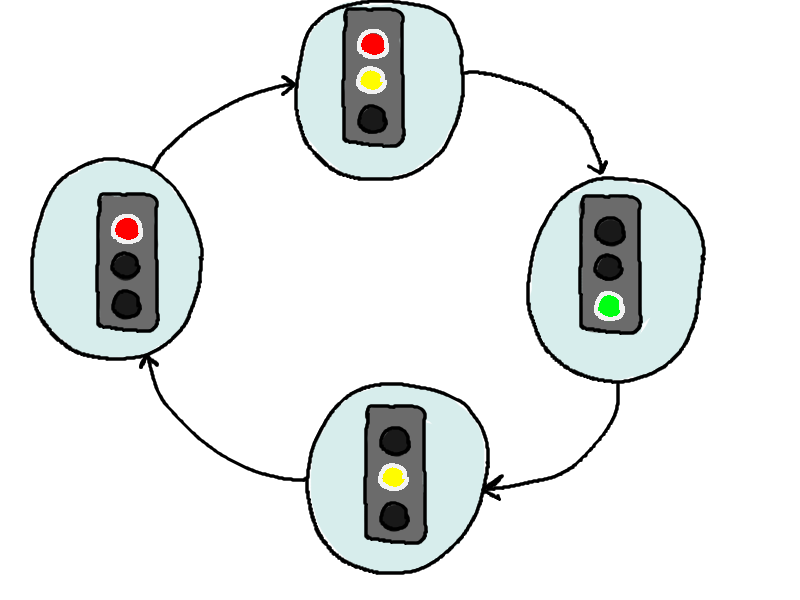
\includegraphics[width=\linewidth]{Pictures/Ampel.png} 
\end{figure}
\end{example}

\begin{example}
Das Beispiel mit dem Getränkautomat -- im Arbeitsblatt leer lassen, im Skript für Johannes und Giovanni ergänzen.
\end{example}

\begin{examplesolution}[print=true]
Das ist die Lösung. Ein schöner Automat.
\end{examplesolution}

\begin{question}
Zeichne einen Obstautomat. (Obstautomat genau beschreiben).
\end{question}

\section{Eigenschaften}
\section{Alphabeten, Wörter, Sprachen}

\section{Endliche Automaten -- eine mathematische Formulierung}
\section{Zusammenfassung}


\end{document}